\documentclass[12pt]{article}
\usepackage[utf8]{inputenc}
\usepackage[a4paper,left=4.5cm,right=1cm,top=2.5cm,bottom=2cm]{geometry}
\usepackage[onehalfspacing]{setspace}
\usepackage{graphicx}
\usepackage[ngerman]{babel}
\usepackage[T1]{fontenc}
\usepackage{microtype}
\usepackage{hyphenat}
\usepackage{url}
\usepackage{booktabs}
\usepackage{tabularx}
\usepackage{bibgerm}
\usepackage[hidelinks]{hyperref}
\usepackage{listings}
\usepackage{color}
\usepackage{afterpage}

\definecolor{dkgreen}{rgb}{0,0.6,0}
\definecolor{gray}{rgb}{0.5,0.5,0.5}
\definecolor{mauve}{rgb}{0.58,0,0.82}
 
%Damit wir Quellcode nutzen können.
\usepackage{listings}
\lstset{
	breaklines=true,
	showstringspaces=false,
	basicstyle=\ttfamily\footnotesize,
	keywordstyle=\color{blue},          % keyword style
  	commentstyle=\color{dkgreen},       % comment style
  	stringstyle=\color{mauve}         % string literal style
}
%Sprache Festelegen
\lstset{language=C}

\title{Intelligenter Labyrinth-Roboter}
\parindent0pt

\begin{document}
\newgeometry{
  left=3cm,
  right=3cm,
  top=2.5cm,
  bottom=2cm,
  bindingoffset=5mm
}
\begin{titlepage}
	\centering
	
\includegraphics[width=0.15\textwidth]{images/sg-logo.png}\par\vspace{1cm}
	{\scshape\LARGE Söderblom Gymnasium \par}
	\vspace{1cm}
	{\scshape\Large Projektdokumentation\par}
	\vspace{1.5cm}
	{\huge\bfseries Intelligenter Labyrinth-Roboter\par}
	\vspace{1.5cm}
	{\Large Jan Beckschewe und Jan Reimer \par}
	\vspace{1.5cm}
	Fachlehrer: Herr Salloch \par
    \vspace{0.5cm}
    Verfasser: Jan Reimer \par
    \vspace{1cm}
	Schuljahr 2016/17 \par
    
	\vfill

	{\large \today\par}
\end{titlepage}
\tableofcontents
\thispagestyle{empty}
\restoregeometry
\newpage
\setcounter{page}{3}
\section{Einleitung}
\paragraph{Allgemein} Robotik ist ein Feld mit vielen Anwendungsmöglichkeiten. Von Militärrobotern bis zu Robotern die Menschen aus Trümmern helfen, aber auch bei gewöhnlichen Dingen wie im Haushalt spielt die Robotik eine immer größer werdende Rolle. Viele Menschen sind an Robotik interessiert, jedoch gibt es Probleme die im Weg stehen: ungeeignete Umgebung und ungenaue Sensoren erschweren den Einsatz erheblich.  

Das Labyrinth besteht aus dünnem schwarzen Klebeband das auf einer weißen Tapete angebracht ist. Um das problemlose abfahren des Labyrinths zu ermöglichen müssen mehrere Faktoren beachtet werden: Bewegungskontrolle in Kombination mit Sensorik, Lösungsalgorithmen für das Labyrinth sowie das Design des Fahrzeugs.

\paragraph{Zielsetzung} Unser Ziel war es einen intelligenten, kleinen und autonomen Roboter zu bauen der ein beliebiges Labyrinth lösen kann in dem er den kürzesten/schnellsten weg zum Ziel findet. Diese Dokumentation wird die notwendige Hardware erklären, angefangen mit dem Mikrocontroller bis zur Auswahl des Akkus. 

\paragraph{Was ist ein Mikrocontroller?} Ein Mikrocontroller ist ein kleiner Computer in einem einzigen integrierten Schaltkreis (englisch integrated circuit, kurz IC). In der modernen Fachsprache werden Mikrocontroller als 'system on a chip', Ein-Chip-System oder auch kurz als SoC bezeichnet. Ein Mikrocontroller beinhaltet einen oder mehrere CPUs (Prozessoren) sowie Speicher und programmierbare I/O Schnittstellen. Außerdem ist oft Programmspeicher, RAM und komplexe Peripherie wie USB- (Universal Serial Bus), I$^2$C- (Inter-Integrated Circuit) Schnittstellen verbaut. Microcontroller sind für den Einsatz in 'embedded applications' (deutsch: eingebettete Systeme) entworfen, im Gegensatz zu Mikroprozessoren die in PCs verwendet werden.

Mikrocontroller werden in automatisch kontrollierten Geräten wie in Motor\hyp Kontrollsystemen, medizinische Implantaten, Fernbedienungen, Elektrowerkzeug, Spielzeug und in vielen anderen embedded systems benutzt. Die ständige Reduktion der Größe und Kosten von Mikrocontrollern macht es technisch und wirtschaftlich möglich immer mehr Geräte und Prozesse digital zu steuern. Mixed signal Microcontroller sind weitverbreitet, um analoge Komponenten zu integrieren, das ist notwendig um nicht digitale elektronische Systeme zu steuern.

Manche Mikrocontroller benutzen lediglich 4-bit Binärwörter und laufen ein sehr geringen Frequenzen um den Stromverbrauch zu senken (einstellige Milliwatt oder Microwatt). Der Stromverbrauch im 'sleep' Zustand (CPU clock und der Großteil der Peripherie ist abgeschaltet) bei wenigen Nanowatt das macht sie perfekt für Anwendungen mit Batteriebetrieb.
\section{Theorie}
\subsection{Hardware}
\paragraph{Arduino Uno Rev.3} Der Arduino Uno ist ein Mikrocontroller Board das auf dem 8-bit ATmega328P basiert er hat 14 digitale I/O pins, 6 analoge Eingänge, eine USB Schnittstelle, einen Stromanschluss, einen ICSP header und einen reset Knopf. Sobald man eine Stromquelle über USB, mit AC zu DC Adapter an die Steckdose  oder einfach mit einer Batterie anschließt kann es los gehen. Man kann sich mit dem Uno austoben ohne viel Angst zu haben etwas falsch zu machen im schlimmsten Fall tauscht man den Chip für wenige Euro aus.

\begin{figure}[thb]
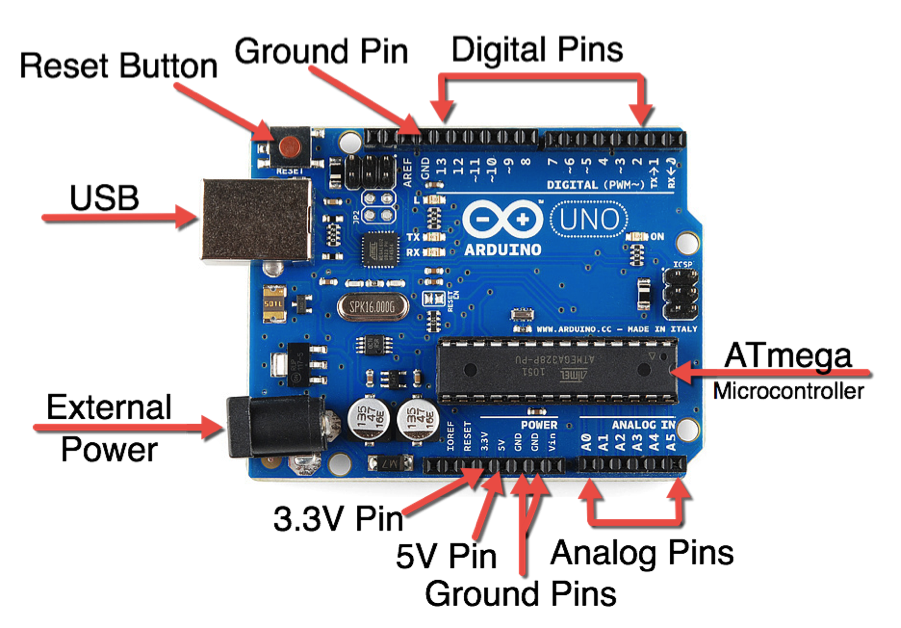
\includegraphics[width=1\textwidth]{images/ArduinoParts.png}
\caption{Arduino Uno \cite{arduino-front}}
\end{figure}

\begin{table}[ht]
\caption{Spezifikationen des Arduino Uno \label{tab:table_label}}
\begin{tabularx}{\columnwidth}{XXl}
  Mikrocontroller&ATmega328p\\
  \hline
  Betriebsspannung&5V\\
  \hline
  Eingangsspannung&6-20V\\
  \hline
  Digitale I/O Pins&14\\
  \hline
  Analoge Eingangs Pins&6\\
  \hline
  DC Strom pro I/O Pin&20 mA\\
  \hline
  DC Strom pro 3.3V Pin&50 mA\\
  \hline
  Flash Memory&32 KB\\
  \hline
  Clock Speed&16 MHz\\
\end{tabularx}
\end{table}

\paragraph{Arduino Motor Shield Rev.3} Der Arduino Motor Shield basiert auf dem L298 Dual-Vollbrücken-Motortreiber und ist entworfen um mit induktiven Ladungen umzugehen die beispielsweise von unseren Motoren erzeugt werden. Der Motor Shield ermöglicht es die Geschwindigkeit und Richtung von beiden DC Motoren eigenständig zu regulieren.

\vspace{0.5cm}
\begin{figure}[thb]
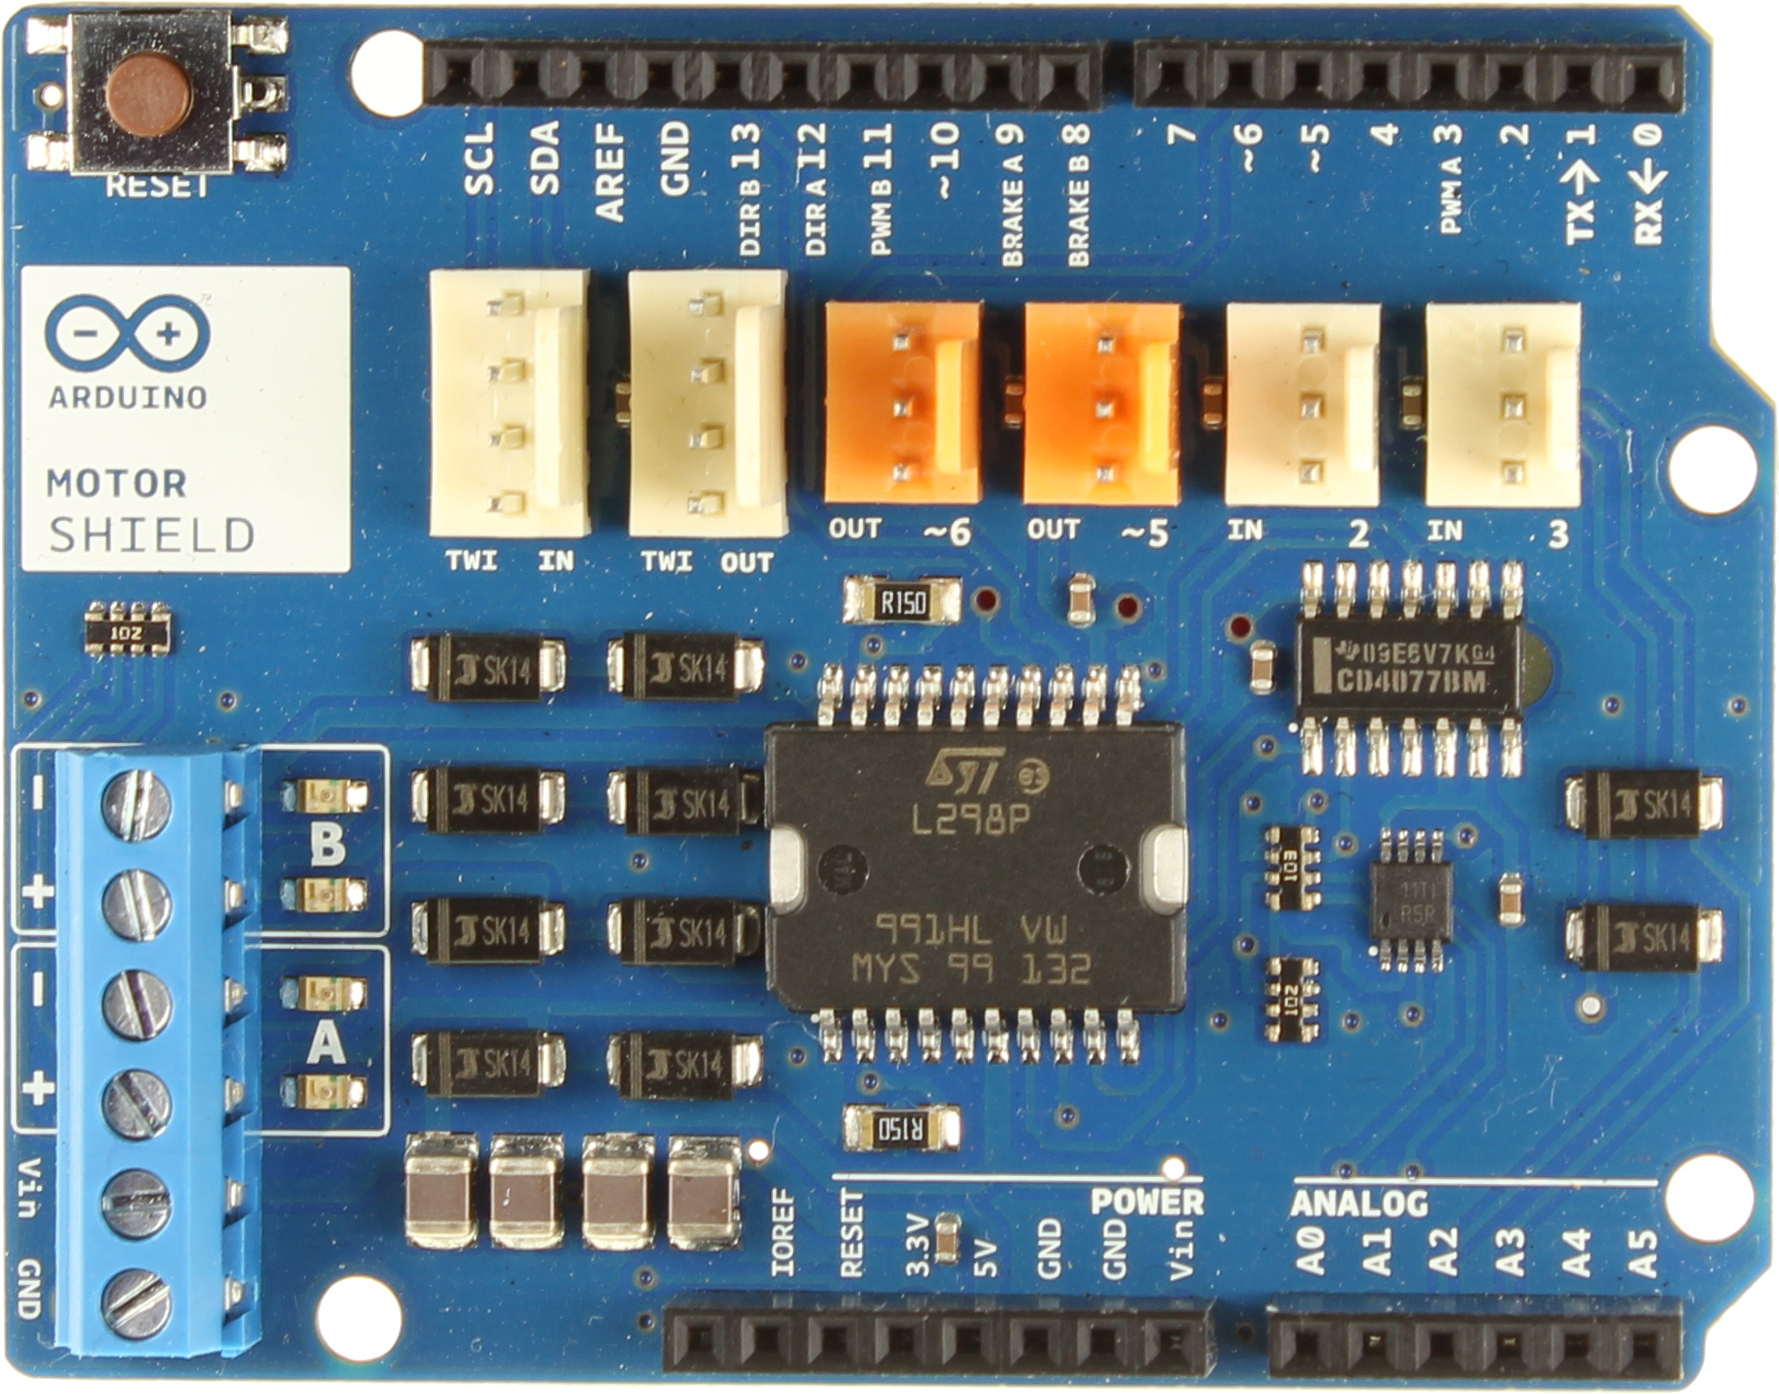
\includegraphics[width=0.6\textwidth]{images/MotorShield_Front.jpg}\par
\caption{Arduino Motor Shield \cite{motorShield-front}}
\end{figure}

\paragraph{Mini Roboter Rover Chassis Kit} Wir haben uns entschieden einen Bausatz zu benutzen um uns das anfängliche Hardware Chaos zu ersparen. Das Kit enthält: 2 Räder, 2 DC Zahnrad Motoren, ein Stützrad, ein Metall Chassis und eine Metallplatte mit Befestigungen.

Da der Aufbau der in der Betriebsanleitung empfohlen ist nicht für unsere Zwecke geeignet ist, haben wir uns entschlossen die Metallplatte an der Unterseite des Autos zu befestigen um die Sensoren möglichst nah an der Drehachse zu verbauen zudem haben wir das Stützrad weiter vorne angebracht um die Stabilität des Fahrzeugs zu verbessern. Die DC Plastik Zahnrad Motoren sind nicht besonders stark und scheitern am kleinsten Hindernis dennoch sind sie für unsere Einsatzzwecke brauchbar. Das Fahrzeug wird durch eine Powerbank mit Strom versorgt.

\vspace{0.5cm}

\begin{figure}[thb]
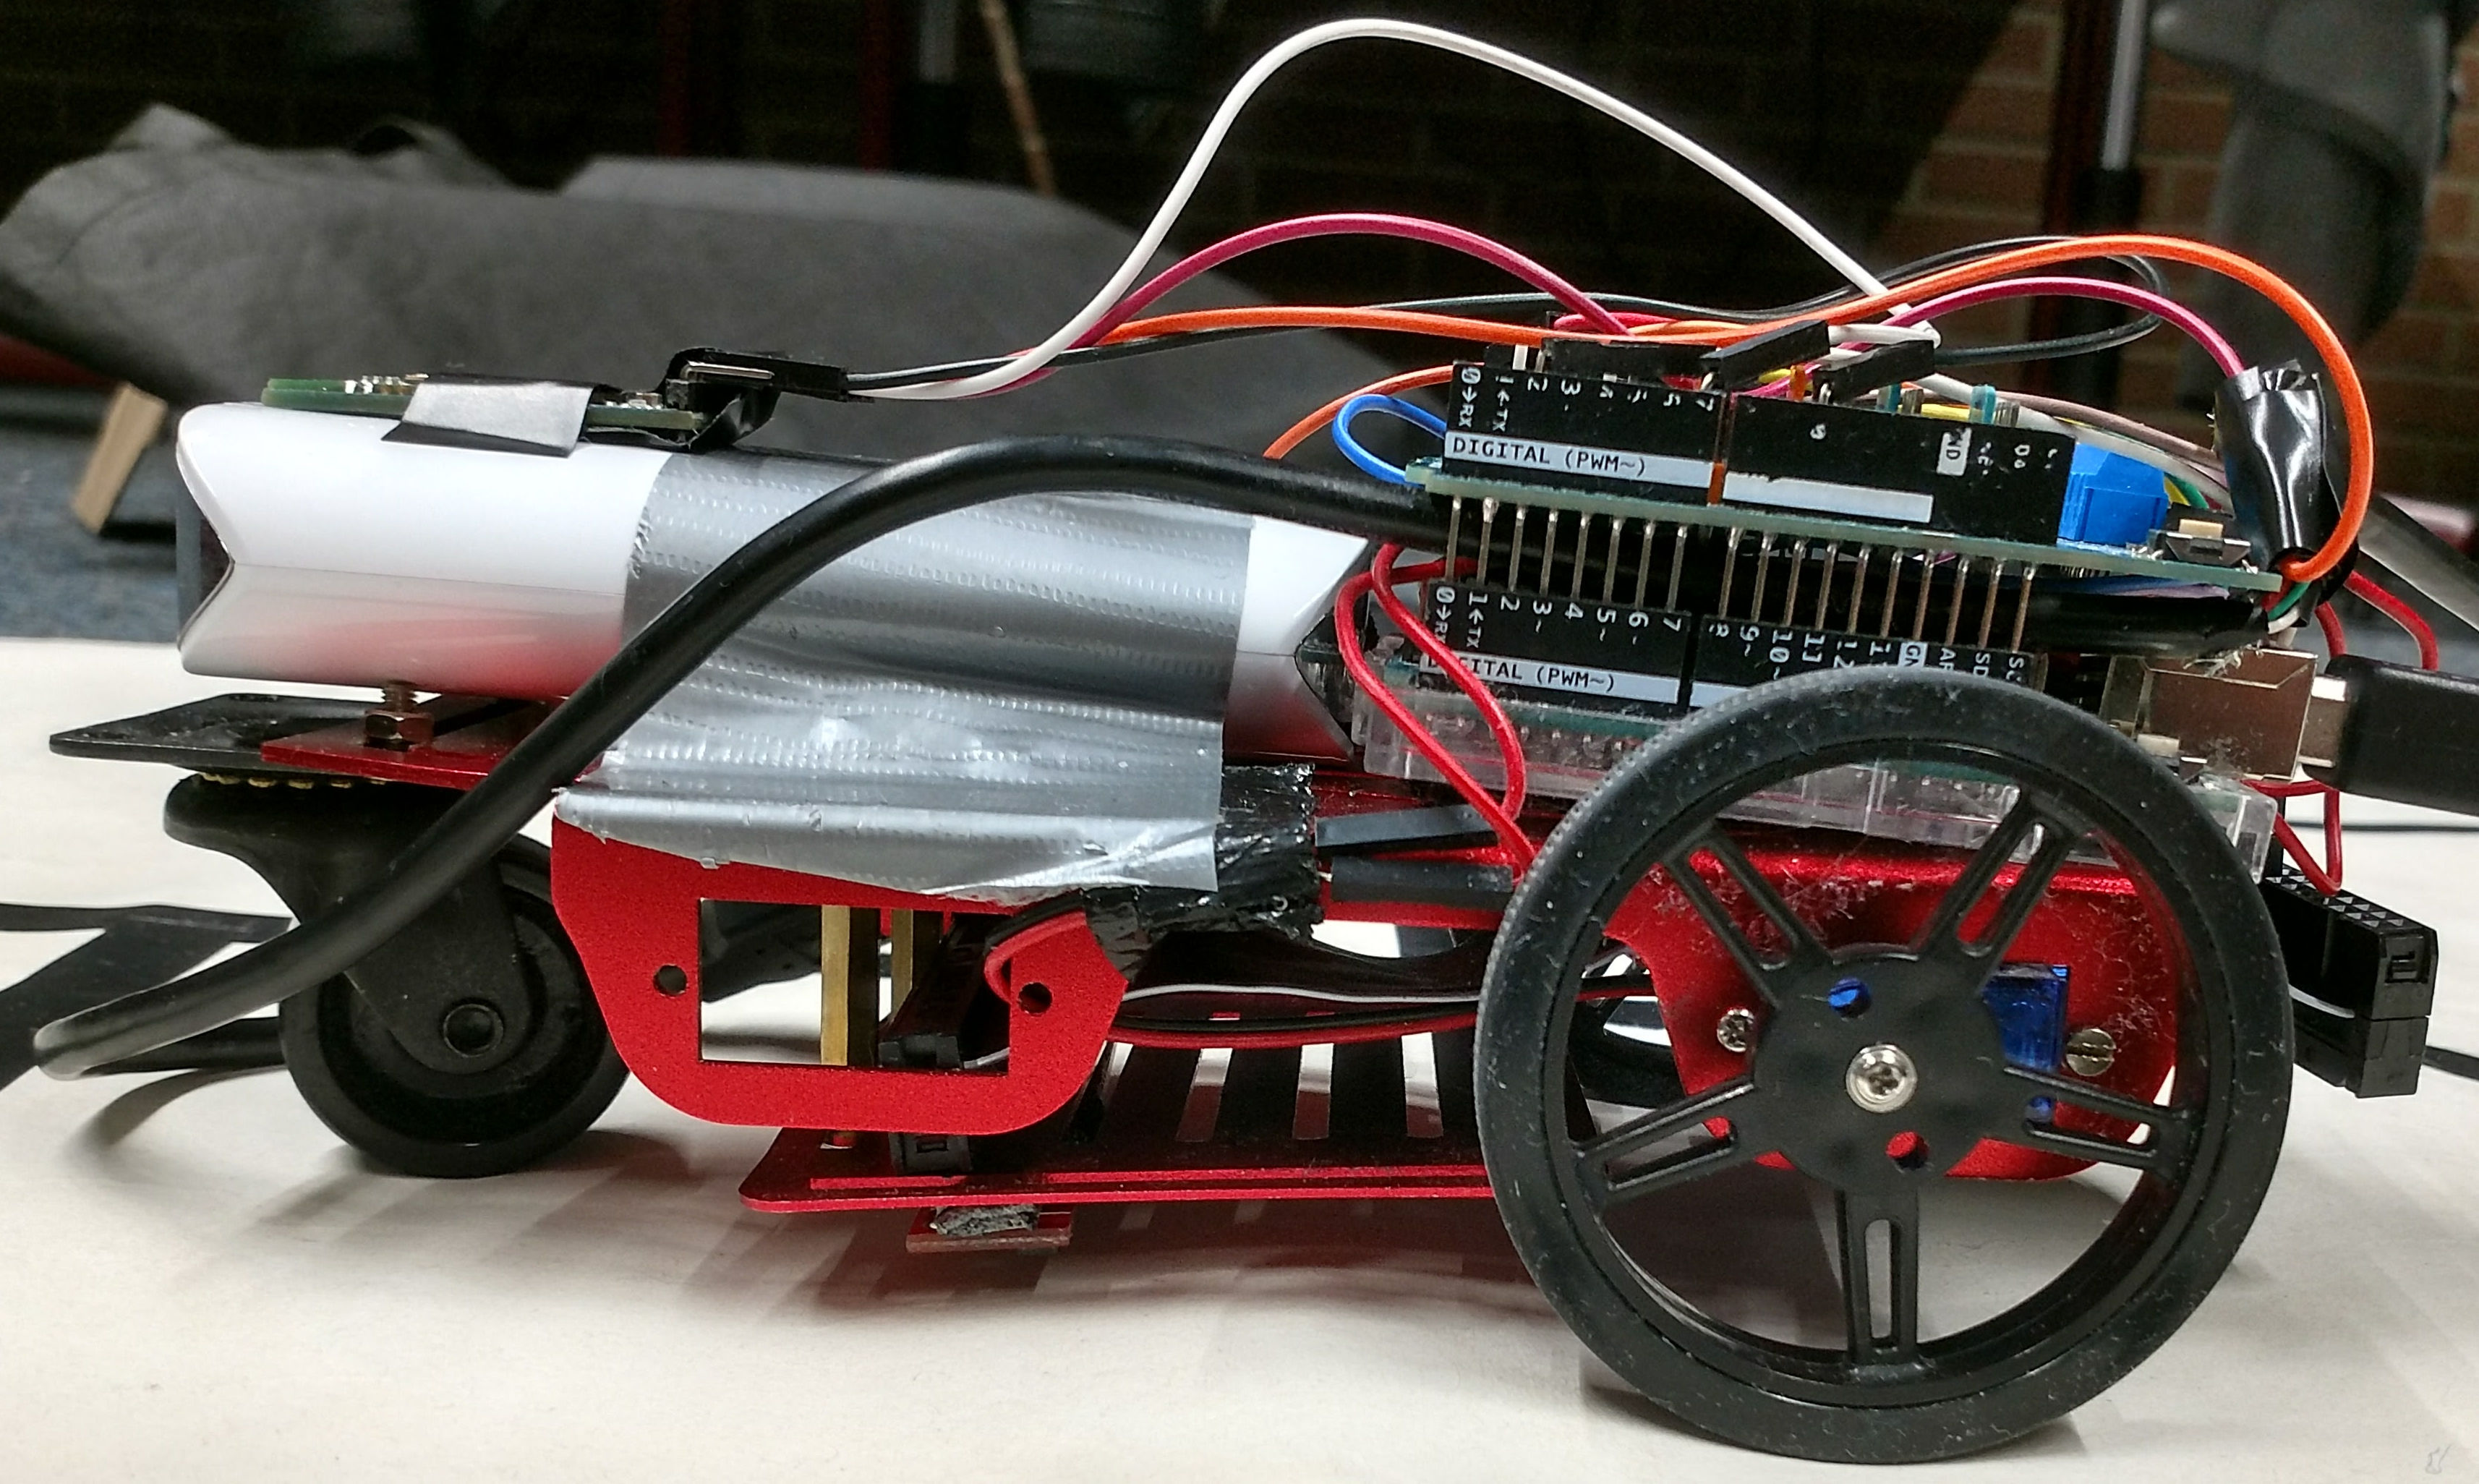
\includegraphics[width=1\textwidth]{images/vehicle_side_small.jpg}
\caption{Aufbau des Roboters}
\end{figure}

\paragraph{QTR-8A Reflexions-Sensoren-Array} Der QTR-8A ist zwar als Linien Sensor entworfen und wird auch so von uns genutzt, jedoch kann man ihn auch als Näherungssensor oder auch einfach als Reflexionssensor. Auf dem Modul befinden sich acht Infrarotstrahler/Infrarotempfänger (Phototransistoren) Paare in gleichmäßigen Intervallen. Jeder Phototransistor ist mit einem 'pull-up' Widerstand verbunden um die Spannung zu verteilen. Jeder angeschlossene Sensor gibt eigenständig eine Analoge Spannung zurück die zwischen 0V und 5V liegt. Geringere Spannung deutet auf eine höhere Reflexion hin.

Der Sensor kann sehr gut zwischen schwarz und weiß unterscheiden, weshalb er sich gut für den Roboter eignet, im Nachhinein wäre ein Sensor mit I$^2$C Anschluss besser gewesen da man sich so einige Kabel sparen kann.
\begin{figure}[thb]
\vspace{0.5cm}
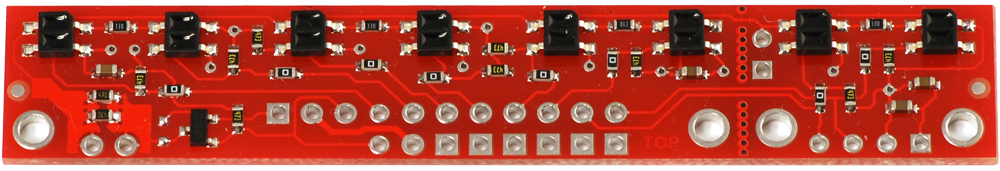
\includegraphics[width=1\textwidth]{images/QTR-8A.jpg}\par
\caption{QTR-8A Sensor\cite{QTR8A-front}}
\end{figure}

\paragraph{SH-HC-08 Bluetooth 4.0 BLE Modul} Der HC-08 ist ein Bluetooth 4.0 Modul. Das Modul benutzt einen Texas Instruments CC2541 Chip der AT Kommandos unterstützt. Man kann die 'baud rate' des Serial ports, den Anzeigenamen des Geräts und das Passwort ändern. Das Bluetooth Modul wird zur Kommunikation zwischen Android Smartphone und Roboter benutzt. Das Modul hat zunächst nicht funktioniert da der Spannungsabfall bei den Pins des Arduino schon zu groß war, deshalb haben wir kurzerhand das USB-Kabel durchgetrennt und das Modul direkt an die Stromversorgung angeschlossen
\subsection{Verwendete Libraries}
\paragraph{Pololu QTR Reflectance Sensors}
\cite{QTR}
Um die Library benutzen zu können muss zunächst ein QTRSensorsAnalog Objekt initialisiert werden. Das Ob jekt gibt einem die Möglichkeit auf die Funktionen der Library zuzugreifen die das Einlesen von Sensordaten ermöglichen. Die Library gibt einem Zugriff auf die rohen Sensordaten sowie 'high level' Funktionen wie das kalibrieren und das Einlesen einer Linie. 

\begin{lstlisting} [caption={Initialisierung des Sensors}] 
QTRSensorsAnalog qtra(sensorPins, sizeof(sensorPins), 4, 2);
unsigned int sensorValues[sizeof(sensorPins)];
\end{lstlisting}

\paragraph{SoftwareSerial Library} \cite{SoftwareSerial}
Die Arduino unterstützt native serielle Kommunikation auf den digitalen Pins 0 und 1. Diese native serielle Unterstützung wird durch den eingebauten 'Universal asynchronous receiver/transmitter' ermöglicht. Die SoftwareSerial Library emuliert die serielle Kommunikation an anderen digitalen Pins des Arduino. Wir haben uns das zunutze gemacht um das Bluetooth Modul an andere digitale Pins anzuschließen. 

\section{Praxis}
\subsection{Anleitung zur Benutzung}
Zur Benutzung benötigen Sie ein 2D-Labyrinth das aus schwarzen Linien auf weißen Untergrund besteht. Achten Sie darauf:
\begin{itemize}
\item Das der Roboter genug Platz zum Wenden hat
\item Das Labyrinth keine Schleifen beinhaltet
\item Der Roboter das Labyrinth nicht verlasen kann
\item Sie das Ziel wie in Abbildung 5 mit einem ausreichend großen schwarzen Kasten markieren
\end{itemize}
Installieren Sie die App aus der Repository\cite{Repo} und stellen Sie sicher das der Akku des Roboters geladen ist. Stellen Sie den Roboter auf irgendeine Linie und stecken Sie das Kabel in die Powerbank. Der Roboter kalibriert sich nun selbst. Öffnen Sie die App und warten Sie bis der Roboter sich verbindet. Drücken Sie auf Start und der Roboter fängt an zu fahren nachdem der Roboter das Ziel erreicht hat stellen Sie in wieder auf den Ausgangspunkt. Der Roboter wird dann den schnellsten/kürzesten Weg zum Ziel fahren. Dieser Vorgang kann beliebig oft wiederholt werden indem man den Roboter nach erreichen des Ziels erneut an den Ausgangspunkt stellt. Will man den Ausgangspunkt ändern stellt man den Roboter auf einen anderen Teil des Labyrinths und drückt die Reset-Taste. Der Roboter wird nun die obigen Schritte erneut durchlaufen.

\begin{figure}[thb]
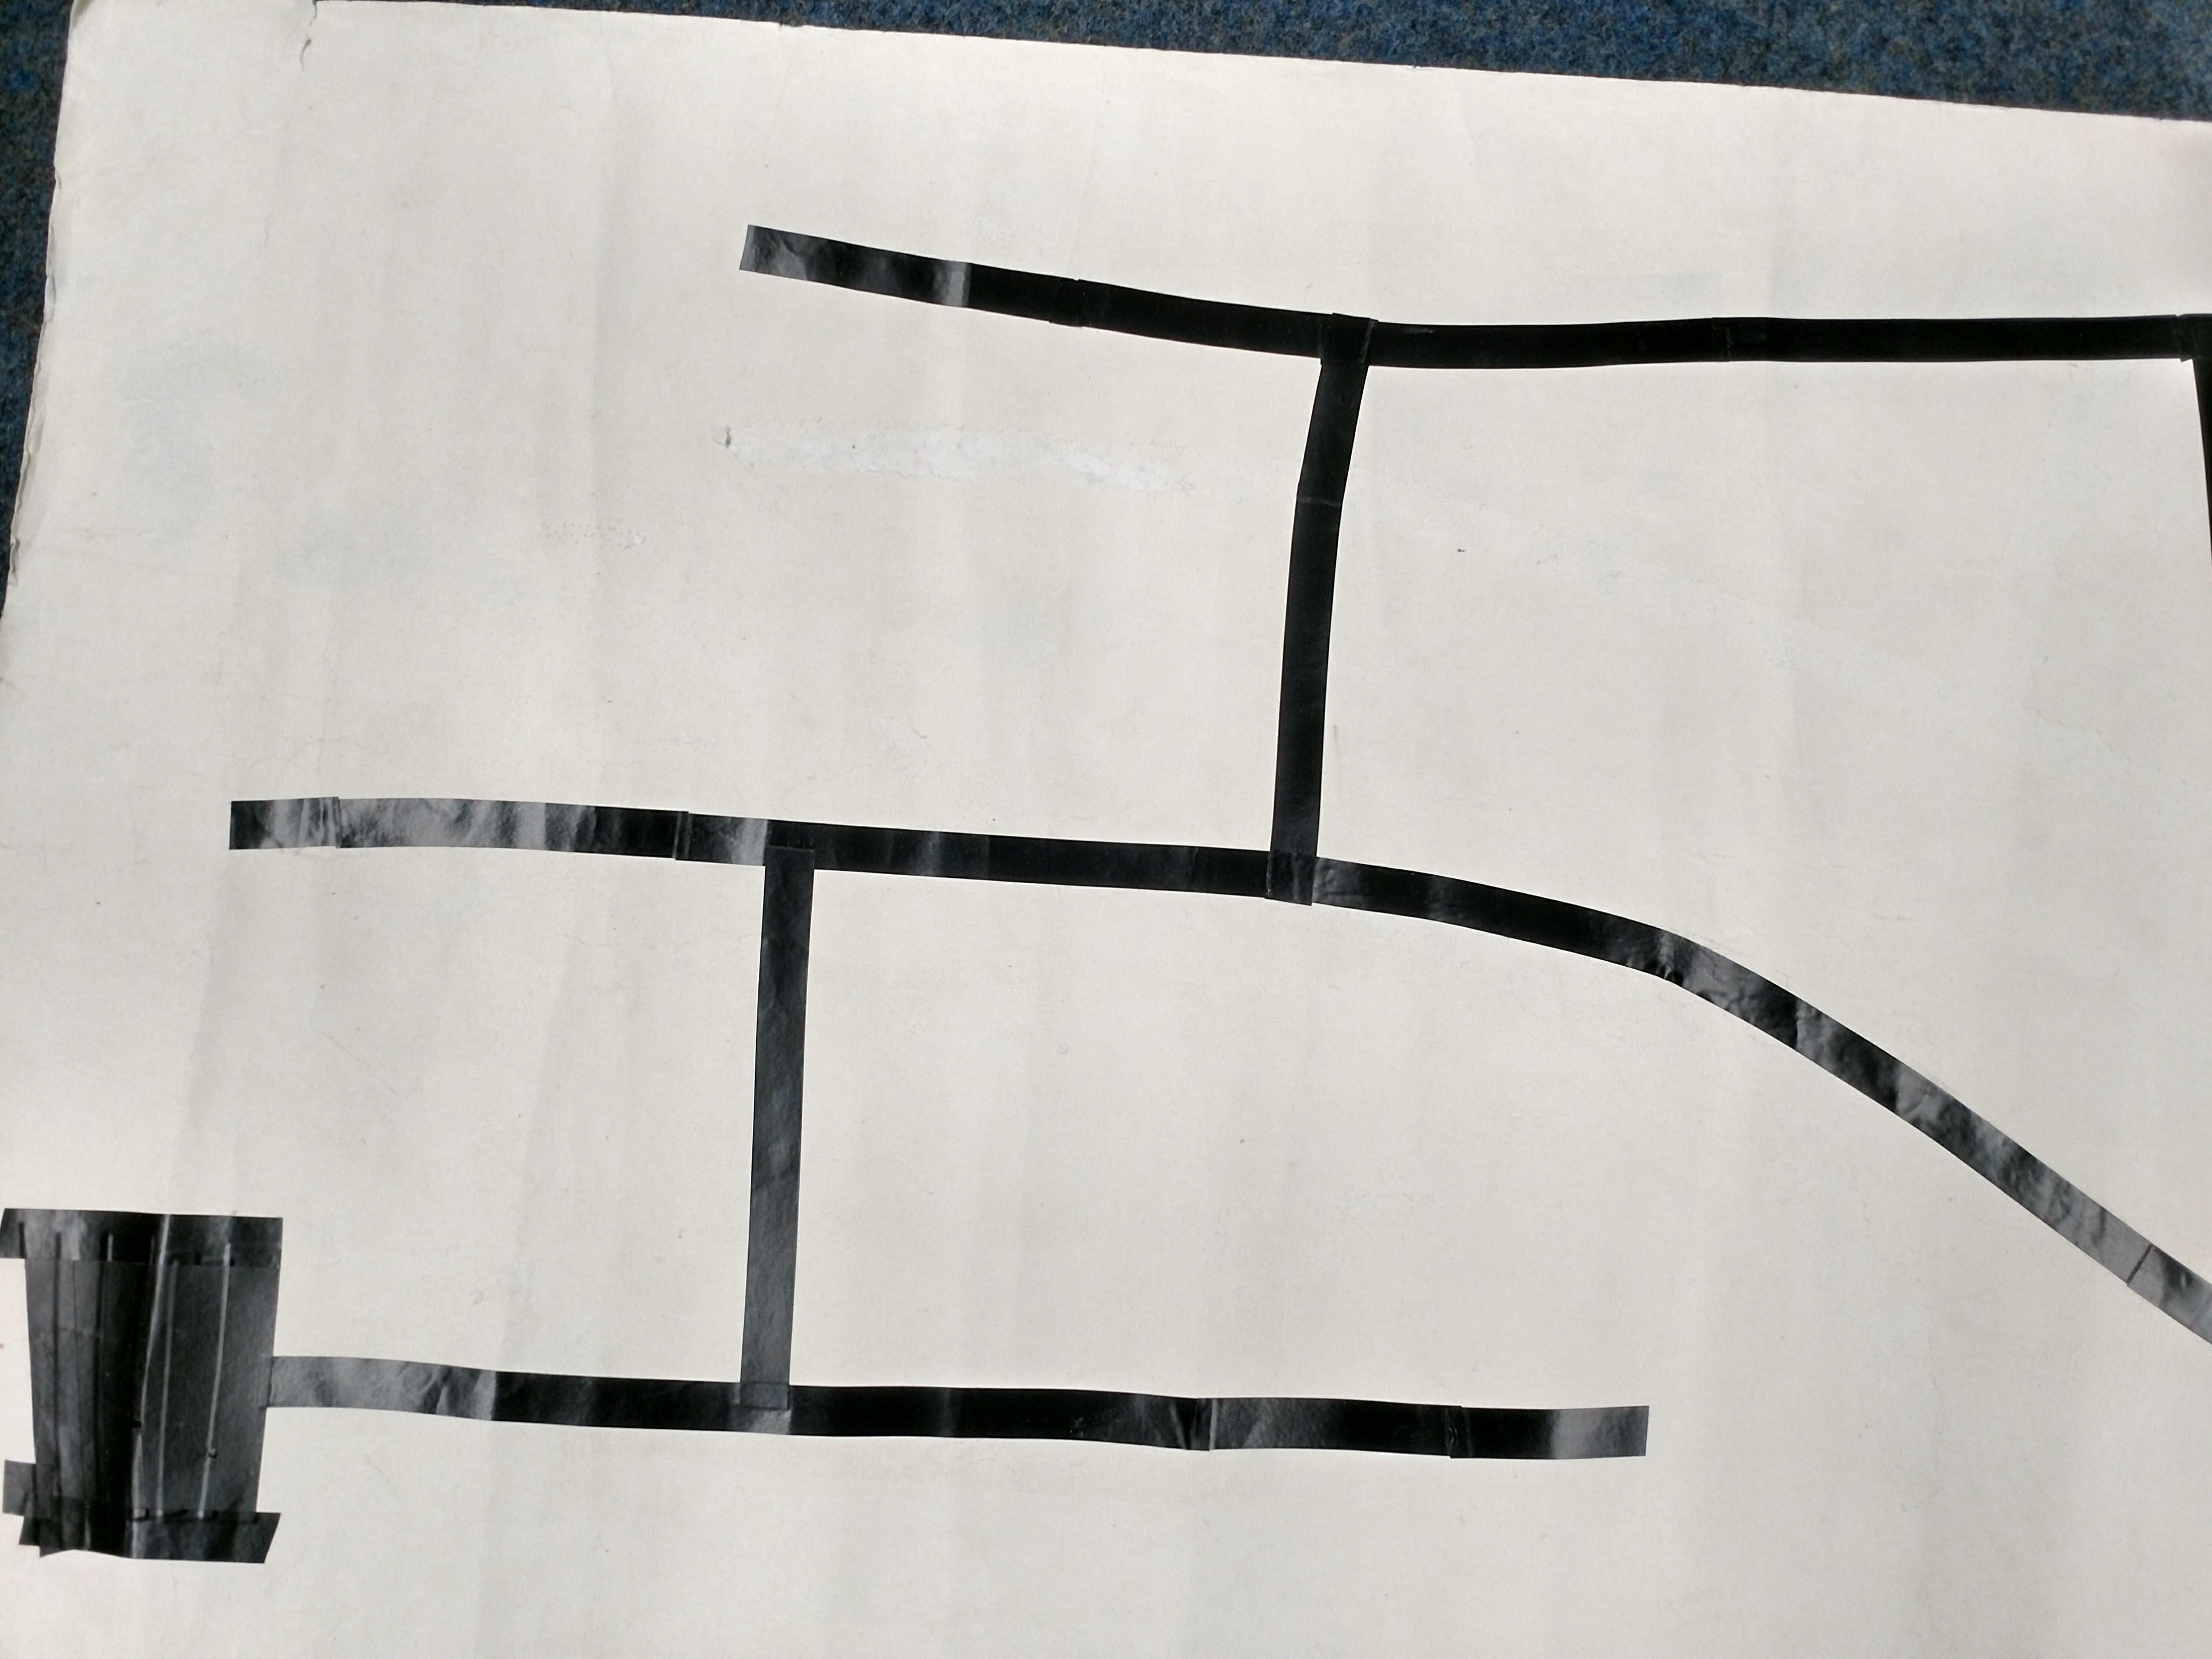
\includegraphics[width=1\textwidth]{images/line_path.jpg}
\caption{Beispiel Labyrinth}
\end{figure}

\subsection{PD-Regler}
\paragraph{Anfängliche Probleme} Eine der ersten Aufgaben der wir uns stellen mussten war das Abfahren einer Linie wobei das Zusammenspiel zwischen Sensorik und Motoren besonders wichtig ist. Doch bevor wir uns diesem ersten Problem widmen konnten hatten wir mehrere Probleme: Zwei Sensoren gaben keine Werte zurück, die Sensoren waren zu weit vom Boden entfernt und das Klebeband was wir als erstes verwendet haben war ungeeignet. Das Klebeband war schnell ausgewechselt und nach einem Umbau des Roboters war auch die Entfernung der Sensoren kein Problem mehr. Die zwei nicht funktionierende Sensoren beschäftigten uns jedoch für eine längere Zeit. Nachdem nach geraumer Zeit falschen Code und defekte Hardware ausschließen konnten haben wir festgestellt das es Pins gibt die immer vom Shield verwendet werden um Spezialfunktionen des Shield wie Richtung und Geschwindigkeit von den Motoren. Da die Funktion (Strommessung) der beiden  Pins für unser Projekt nicht zu gebrauchen ist, bogen wir die Verbindungsstellen des Shields ab und verbanden die beiden Sensoren direkt mit dem Arduino.
\paragraph{Umsetzung} Ungenauigkeiten im Labyrinth und Unebenheiten verhindern es das man den Roboter nur geradeaus fahren lassen kann, da er sonst schnell die Spur verliert und man eventuell auch Kurven fahren möchte. Deshalb muss ein Regler implementiert werden der selbständig die Geschwindigkeiten der Motoren anpasst um den Roboter möglichst mittig auf der Strecke der zu halten. 

Der Roboter kann mithilfe der Infrarotsensoren bestimmen wie er im Labyrinth steht. Die readLine() Methode der Library gibt bei 6 Sensoren einen Wert zwischen 0 und 5000 zurück mithilfe dieser Methode haben wir einen PD  Regler implementiert der anhand der jetzigen Position (proportional) und der letzten Position (derivative) seine Motorgeschwindigkeiten anpasst. PD Regler kommen zum Beispiel bei Klimaanlagen vor damit wird verhindert das die Klimaanlage den Raum nicht immer periodisch unterkühlt und sorgt dafür das die Wunschtemperatur im Raum herrscht.
\begin{lstlisting} [caption={PD Regler Implementation}] 
// PD loop constants
const float proportionalConst = 0.2f;
const float derivateConst = 1.0f;

posPropotionalToMid = sensorPosition - 2500;

motorSpeed = proportionalConst * posPropotionalToMid + derivateConst * (posPropotionalToMid - lastError);
lastError = posPropotionalToMid;

moveBothMotors(maxMotorSpeed - motorSpeed, forward, maxMotorSpeed + motorSpeed, forward);
\end{lstlisting}
Wie man im Code sieht werden zwei Konstanten initialisiert die den Einfluss der jetzigen und vorherigen Position auf die Motorlenkung bestimmen. Die Konstanten müssen dem Gewicht des Roboters und der Leistungsfähigkeit der Motoren angepasst werden hat man aber die richtigen Werte gefunden folgt der Roboter dem Pfad perfekt.

\subsection{Abbiegen} Das nächste Problem mit dem wir uns beschäftigt haben ist das Abbiegen. Es gibt beim Abbiegen mehrere Probleme:
\begin{itemize}
\item Wie muss man abbiegen um das Labyrinth gründlich und effizient zu durchfahren?
\item Wie erkennt man eine Kreuzung?
\end{itemize}
\paragraph{Durchfahren des Labyrinths} Die erste Frage war theoretisch schnell gelöst, der Roboter muss die Links-Hand-Regel beachten, das heißt  er hält sich immer an linken Wand. Daraus schlussfolgert man folgende Priorität für die Abbiegungen: Wenn du nach links abbiegen kannst biege nach links ab, ist das nicht möglich fahre geradeaus ist das auch nicht möglich biege rechts ab.
\begin{lstlisting} [caption={Linke-Hand-Regel Implementation}]
if (isEachDiversionOnCrossing[left])
{
    direction = left;
}
else if (isEachDiversionOnCrossing[forward])
{
    direction = forward;
}
else
{
    direction = right;
}
\end{lstlisting}

\paragraph{Erkennung der Kreuzung} Die Sackgasse ist die einfachste 'Kreuzung' denn es ist die einzige Situation wo die Sensorwerte sich von '001100' zu '000000' verändern (wobei 1 für eine Linie unter dem Sensor steht und 0 für weißen Untergrund). Wird eine Sackgasse erkannt dreht sich der Roboter um. 

\begin{lstlisting} [caption={Erkennen von Sackgassen}]
// dead end
else if (getNumberOfCurrentlyWhiteSensors() == sizeof(sensorPins))
{
    direction = backward;
    storeTurnToPath();
}
\end{lstlisting}
Der nächste Fall ist die Unterscheidung zwischen einer Kreuzung wo man nur rechts abbiegen kann und einer Kreuzung wo man gerade und rechts fahren kann. Beide zeigen zu Anfang das Muster '000111' aber wie weiß man welcher Fall vorliegt.

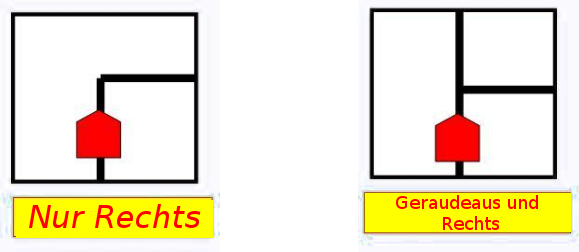
\includegraphics[width=1\textwidth]{images/case_right.png}

Die Lösung ist einfach man fährt einfach ein wenig weiter und liest die Sensoren erneut aus. Sind die Sensorwerte nach erneutem einlesen '000000' ist nur eine rechte Abbiegung vorhanden. Sind die Sensorwerte '001100' kann man auch geradeaus fahren und das gleiche gilt auch anders herum für linke Abbiegungen.

\begin{lstlisting} [caption={Erkennen von Abbiegungen}]
void checkForDiversions()
{
    if (sensorValues[sizeof(sensorPins) - 1] > threshold)
    {
        isEachDiversionOnCrossing[right] = true;
    }
    if (sensorValues[0] > threshold)
    {
        isEachDiversionOnCrossing[left] = true;
    }
}
\end{lstlisting}

\begin{lstlisting} [caption={Erkennung von geraden Strecken durch vorwärts fahren}]
checkForDiversions();
if (isEachDiversionOnCrossing[left] || isEachDiversionOnCrossing[right])
    {
        direction = diversionChecking;
        startFurtherDiversionCheckingTime();
    }
\end{lstlisting}
Der letzte zu beachtende Fall ist das erreichen vom Ende des Labyrinths wenn alle sechs Sensoren schwarzen Untergrund auch nach Vorwärtsfahren einen komplett schwarzen Untergrund erkennen hält der Roboter an.
\begin{lstlisting} [caption={Erkennung des Ziels}]
if (getNumberOfCurrentlyWhiteSensors() == 0)
{
    direction = none;
}
\end{lstlisting}

\subsection{Lösen des Labyrinths}
\paragraph{Welche Schritte müssen zum Lösen des Labyrinths durchgeführt werden?} 
Es gibt im wesentlichen 2 Schritte. Der erste ist es das Labyrinth zu durchfahren und das Ende zu finden. Der zweite ist es den Pfad so zu optimieren das der Roboter den schnellsten Weg durch das Labyrinth findet

\paragraph{Das Lösen}
Um das Lösen des Labyrinth zu erläutern werden ich  ein einfaches Beispiel Labyrinth lösen. Der rote Punkt steht für den Startpunkt des Roboters, der schwarze Kasten zeigt das Ende an. Wenn das Labyrinth mit der Links-Hand-Regel abgefahren wird ist der Pfad 'LBLLBSR'.
\par
L = Links
R = Rechts
S = Geradeaus
B = Umdrehen

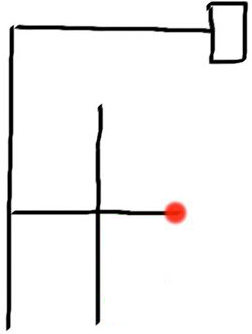
\includegraphics[width=0.8 \textwidth]{images/example_maze.png}

Wie kann man jetzt diesen Pfad jetzt zum schnellsten Weg 'SSR' umwandeln. Für den Anfang stellen wir erst mal fest wo wir falsch abgebogen sind. Ein 'B' signalisiert das der Roboter sich gedreht hat was bedeutet das er auf den falschen Pfad gefahren ist. Um den Pfad zu optimieren müssen wir das B durch Substitution entfernen.

Zuerst schauen wir uns die ersten drei Abbiegungen im Pfad 'LSBLLBSR'. Diese Bewegungen sieht man im Foto.

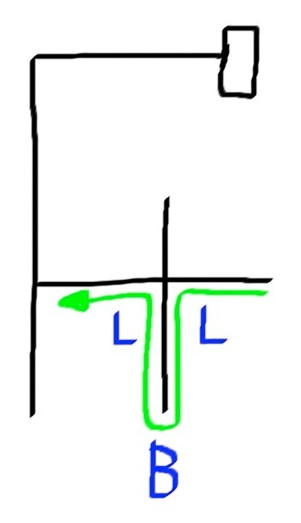
\includegraphics[width=0.6\textwidth]{images/first_three_turns.jpg}

Statt links abzubiegen dann umzukehren und nochmal links abzubiegen kann man auch einfach links fahren. Also ist LBL =S. Das ist ein Beispiel einer Optimierung aber hier ist die ganze Liste:\par
LBR = B \hspace{0.2cm} LBS = R \hspace{0.2cm} RBL = B \hspace{0.2cm} SBL = R \hspace{0.2cm}SBS = B \hspace{0.2cm} LBL = S

Lasst uns jetzt den Pfad optimieren: 'LBLLSBR' wir wissen das LBL=S also ist unser neuer Pfad: 'SLBR'. Wir wissen auch das LBS=R also ist unser neuer Pfad:  
'SRR'. Wie man sieht ist das der schnellste Weg.

Der Roboter optimiert das Labyrinth während des Fahrens. Jedes mal wenn eine Abbiegung gespeichert wird überprüft es ob die letzte Abbiegung ein B war, wenn das zutrifft wird der Pfad optimiert. Man muss mindesten 3 Bewegungen kennen um den Pfad zu optimieren (siehe Listing 9 im Anhang). 

\subsection{Selbstkalibration}
Ein kleines Feature was wir eingebaut haben ist die Selbstkaltbration der Sensoren. In der Kalibrationsphase müssen alle Sensoren auf die Extremwerte der Reflexion eingestellt sein um sich so an die Reflexion des Labyrinths anzupassen. Wir lassen das Fahrzeug also ein paar Mal während der Kalibrationsphase hin und her schwenken so das jeder Sensor auf die Reflexion des Labyrinths eingestellt ist, anschließend dreht sich der Roboter dann soweit das er wieder mittig auf der Linie steht.
\begin{lstlisting} [caption={Implementation der Selbstkalibration}]
void calibrate()
{
    // make half-turns to have values for black and white without holding it
    for (byte i = 0; i <= 100; i++)
    {
        if (i == 0 || i == 60)
        {
            moveBothMotors(150, backward, 150, forward);
        }

        else if (i == 20 || i == 100)
        {
            moveBothMotors(150, forward, 150, backward);
        }

        qtra.calibrate();
}
\end{lstlisting}

\subsection{Android App} In der Endphase des Projekts wollten wir noch eine Android App entwickeln die sich mit dem Bluetooth Modul des Arduino verbindet und dann das Labyrinth an die App sendet um das Labyrinth  und den schnellsten Weg durch auf dem Smartphone darzustellen. Die Verbindung ist zustande gekommen und die Abbiegungen werden auch mithilfe eines dafür entwickelten Protokolls gesendet, die Darstellung des Labyrinths ist jedoch mangelhaft. Man kann den Roboter mit der App starten und stoppen.

\begin{table}[h]
\caption{Protokoll zum senden des Labyrinths \label{tab:table_label}}
\begin{tabularx}{\columnwidth}{XXl}
  
  byte&value\\
  \hline
starting & 255\\
the index & 0 to 245\\
the direction & 250 to 253\\
left & 250\\
forward & 251\\
right & 252\\
backward & 253\\
the time  in 50 ms & 0 to 246 (0  to 12.25 seconds)\\
finishing and requesting response & 254\\
phone saying received & 249\\
phone request start driving & 247\\
phone request stop driving & 248\\
Arduino request clear the maze view on Android & 246\\
  
\end{tabularx}
\end{table}

\newpage
\section{Zusammenfassung} In diesem Projekt wurde das Primärziel erreicht. Der Roboter ist in der Lage ein Labyrinth abzufahren und zu lösen. Jedoch ist kein abfahren eines Labyrinths mit Schleifen vollkommen möglich, da wenn er im schlechtesten Fall dort nur im Kreis fährt. Das Darstellen des Labyrinths auf einem Smartphone funktioniert bei Projektabgabe jedoch noch nicht. Um das Projekt zu vervollständigen müsste die App funktionieren. Weitere Features wären die Implementation eines anderen Lösungsalgorithmen sowie das zurück finden vom Ziel zum Ausgangspunkt. Abschließend lässt sich sagen das Die Projektarbeit gelungen ist und ich mit den Ergebnis zufrieden bin.  

\section{Erklärung der Urheberschaft}

Hiermit versichere ich, dass ich die vorliegende Arbeit
ohne Hilfe Dritter und ohne Benutzung anderer als der angegebenen
Hilfsmittel angefertigt habe; die aus fremden Quellen direkt oder
indirekt übernommenen Gedanken sind als solche kenntlich gemacht.


\vspace{4cm}
\rule{\textwidth}{1pt}
\hspace{2cm} Ort, Datum \hfill Unterschrift \hspace{2cm}

\newpage
\bibliographystyle{gerplain}
\bibliography{literatur}


 





\newpage
\begin{lstlisting} [caption={Implmentierung der Vereinfachung}]
void simplifyMaze()
{
    if (pathLength < 3 || simplePath[pathLength - 2].direction != backward)
    {
        return;
    }

    int totalAngle = 0;

    for (byte i = 1; i <= 3; i++)
    {
        switch (simplePath[pathLength - i].direction)
        {
        case right:
            totalAngle += 90;
            break;
        case left:
            totalAngle += 270;
            break;
        case backward:
            totalAngle += 180;
            break;
        }
    }
    totalAngle = totalAngle % 360;.
    switch (totalAngle)
    {
    case 0:
        simplePath[pathLength - 3].direction = forward;
        break;
    case 90:
        simplePath[pathLength - 3].direction = right;
        break;
    case 180:
        simplePath[pathLength - 3].direction = backward;
        break;
    case 270:
        simplePath[pathLength - 3].direction = left;
        break;
    }

    simplePath[pathLength - 1].direction = none;
    simplePath[pathLength - 2].direction = none;
    pathLength -= 2;
}
\end{lstlisting}

\end{document}
